\documentclass[9pt,aspectratio=169,xcolor=table]{beamer}

%~~~~~~~~~~~~~~~~~~~~~~~~~~~~~~~~~~~~~~~~~~~~~~~~~~~~~~~~~~~~~~~~~~~~~~~~~~~~~~
% Use roboto Font (recommended)
\usepackage[sfdefault]{roboto}
\usepackage[utf8]{inputenc}
\usepackage[T1]{fontenc}
%~~~~~~~~~~~~~~~~~~~~~~~~~~~~~~~~~~~~~~~~~~~~~~~~~~~~~~~~~~~~~~~~~~~~~~~~~~~~~~

%~~~~~~~~~~~~~~~~~~~~~~~~~~~~~~~~~~~~~~~~~~~~~~~~~~~~~~~~~~~~~~~~~~~~~~~~~~~~~~
% Define where theme files are located. ('/styles')
\usepackage{styles/fluxmacros}
\usefolder{styles}
% Use Flux theme v0.1 beta
% Available style: asphalt, blue, red, green, gray
% "red" is the closest built-in style to maroon; its exact colours are
% overridden with a true maroon palette just below, after the theme loads.
\usetheme[style=red]{flux}
%~~~~~~~~~~~~~~~~~~~~~~~~~~~~~~~~~~~~~~~~~~~~~~~~~~~~~~~~~~~~~~~~~~~~~~~~~~~~~~

%~~~~~~~~~~~~~~~~~~~~~~~~~~~~~~~~~~~~~~~~~~~~~~~~~~~~~~~~~~~~~~~~~~~~~~~~~~~~~~
% SKEE1033 maroon palette override.
% The flux theme's colortheme defines primaryLight/primary/secondary/tertiary
% as plain \definecolor calls (not \providecolor), so simply redefining them
% here, AFTER \usetheme, wins -- xcolor allows redefinition and every
% \setbeamercolor in beamercolorthemeflux.sty was already evaluated against
% these names, so the redefinition propagates everywhere automatically.
\definecolor{primaryLight}{HTML}{9B2242} % lighter maroon -- headers, accents
\definecolor{primary}{HTML}{7B1E3A}      % core maroon -- titles, block headers
\definecolor{secondary}{HTML}{3A5A6B}    % muted teal -- complementary accent
\definecolor{tertiary}{HTML}{8C6A3F}     % warm bronze -- example/third accent
%~~~~~~~~~~~~~~~~~~~~~~~~~~~~~~~~~~~~~~~~~~~~~~~~~~~~~~~~~~~~~~~~~~~~~~~~~~~~~~

%~~~~~~~~~~~~~~~~~~~~~~~~~~~~~~~~~~~~~~~~~~~~~~~~~~~~~~~~~~~~~~~~~~~~~~~~~~~~~~
% Extra packages
\usepackage{booktabs}
\usepackage{colortbl}
\usepackage{ragged2e}
\usepackage{amssymb}
\usepackage{multirow}
\usepackage{tikz}
\usetikzlibrary{arrows.meta, positioning, fit, backgrounds, calc, shapes.geometric}
\setbeamertemplate{itemize items}[square]
\usepackage[scaled=.92]{beramono}
\usepackage{listings}
\usepackage{array}
% Table striping: odd rows white, even rows very light gray.
\definecolor{stripe}{gray}{0.94}
\newcommand{\striped}{\rowcolors{1}{white}{stripe}}
%~~~~~~~~~~~~~~~~~~~~~~~~~~~~~~~~~~~~~~~~~~~~~~~~~~~~~~~~~~~~~~~~~~~~~~~~~~~~~~

%~~~~~~~~~~~~~~~~~~~~~~~~~~~~~~~~~~~~~~~~~~~~~~~~~~~~~~~~~~~~~~~~~~~~~~~~~~~~~~
% Code listing style (lightweight analogue of the book's skpython style).
% This course is Python-only, so Python is set as the lstlisting default via
% \lstset below -- every \begin{lstlisting} needs no language=... of its own.
\definecolor{codebg}{HTML}{FBF2F4}
\definecolor{codegreen}{rgb}{0,0.45,0}
\definecolor{codestring}{rgb}{0.58,0.1,0.2}
\lstdefinestyle{skpython}{
    basicstyle=\ttfamily\footnotesize,
    keywordstyle=\color{primary}\bfseries,
    commentstyle=\itshape\color{codegreen},
    stringstyle=\ttfamily\color{codestring},
    backgroundcolor=\color{codebg},
    breaklines=true,
    keepspaces=true,
    showspaces=false,
    showstringspaces=false,
    frame=single,
    rulecolor=\color{primary!40},
    numbers=none,
}
\lstdefinestyle{skoutput}{
    basicstyle=\ttfamily\footnotesize,
    backgroundcolor=\color{secondary!8},
    breaklines=true,
    keepspaces=true,
    showspaces=false,
    showstringspaces=false,
    frame=single,
    rulecolor=\color{secondary!50},
    numbers=none,
}
\lstset{language=Python, style=skpython}
%~~~~~~~~~~~~~~~~~~~~~~~~~~~~~~~~~~~~~~~~~~~~~~~~~~~~~~~~~~~~~~~~~~~~~~~~~~~~~~

%~~~~~~~~~~~~~~~~~~~~~~~~~~~~~~~~~~~~~~~~~~~~~~~~~~~~~~~~~~~~~~~~~~~~~~~~~~~~~~
% TikZ block styles (kept for visual consistency with ecp01.tex, reused for
% any process/flow diagrams)
\definecolor{cycfill}{HTML}{F3DCE4}
\definecolor{cycline}{HTML}{7B1E3A}
\definecolor{cycdofill}{HTML}{E8EEF0}
\definecolor{cycdoline}{HTML}{3A5A6B}
\tikzset{
  cycstep/.style = {font=\sffamily\small, align=center, rounded corners=2pt,
                     draw=cycline, fill=cycfill, line width=0.7pt,
                     minimum height=7mm, minimum width=20mm, inner sep=3pt},
  cycdo/.style   = {cycstep, fill=cycdofill, draw=cycdoline},
  flow/.style    = {-{Stealth[length=2mm]}, thick, draw=cycline},
}
%~~~~~~~~~~~~~~~~~~~~~~~~~~~~~~~~~~~~~~~~~~~~~~~~~~~~~~~~~~~~~~~~~~~~~~~~~~~~~~

%%%%%%%%%%%%%%%%%%%%%%%%%%%%%%%%%%%
%% SECTION SEPARATOR (ToC recap) %%
%%%%%%%%%%%%%%%%%%%%%%%%%%%%%%%%%%%
\AtBeginSection[]
{
{
    \setbeamercolor{background canvas}{bg=primaryLight!6}
    \begin{frame}[plain]
        \frametitle{Table of Contents}
        \tableofcontents[currentsection]
    \end{frame}
}
}
%%%%%%%%%%%%%%%%%%%%%%%%%%%%%%%%%%%

%~~~~~~~~~~~~~~~~~~~~~~~~~~~~~~~~~~~~~~~~~~~~~~~~~~~~~~~~~~~~~~~~~~~~~~~~~~~~~~
% Information
\title{Your First Python Programs}
\subtitle{\emph{Engineering Computation with Python} --- Chapter 2}
\author{Mun\'{i}m Zabidi}
\institute{\color{primary}Faculty of Electrical Engineering, Universiti Teknologi Malaysia}
\date{\today}
\titlegraphic{assets/logoutmwhite.png}
%~~~~~~~~~~~~~~~~~~~~~~~~~~~~~~~~~~~~~~~~~~~~~~~~~~~~~~~~~~~~~~~~~~~~~~~~~~~~~~

\begin{document}

\titlepage

\begin{frame}{Table of Contents}
    \tableofcontents
\end{frame}

%===============================================================================
\section{Introduction}
%===============================================================================

\begin{frame}{From Paper to the Machine}
    \leavevmode
    Chapter 1 described what programs are and how algorithms are expressed
    on paper. This chapter is where that becomes real.

    \vspace{3mm}
    \begin{block}{What you will do this week}
        Set up the software, type your first Python statements, and watch
        the machine execute them.
    \end{block}

    \vspace{2mm}
    \begin{alertblock}{Why it matters}
        The ideas here --- variables, types, the editor you work in --- are
        small individually, but \alert{everything else in this course is
        written on top of them}.
    \end{alertblock}
\end{frame}

\begin{frame}{A Programming Language Is Like a Natural Language}
    \leavevmode
    Learning Python can be approached the same way you learned a natural
    language: built from a \alert{grammar} and a \alert{dictionary}.

    \vspace{3mm}
    \begin{columns}[t]
        \begin{column}{.33\textwidth}
            \begin{block}{Syntax}
                \small The layout of words and symbols. \\[1mm]
                \emph{Like:} grammar.
            \end{block}
        \end{column}
        \begin{column}{.33\textwidth}
            \begin{block}{Variables}
                \small A stored value, retrieved by name. \\[1mm]
                \emph{Like:} a noun.
            \end{block}
        \end{column}
        \begin{column}{.33\textwidth}
            \begin{block}{Operation}
                \small An action on variables. \\[1mm]
                \emph{Like:} a verb.
            \end{block}
        \end{column}
    \end{columns}

    \vspace{4mm}
    \begin{center}
        \small Syntax is the grammar; variables are the nouns; operations
        are the verbs.
    \end{center}
\end{frame}

\begin{frame}{Every Variable Carries Three Properties}
    \leavevmode
    \begin{columns}[t]
        \begin{column}{.5\textwidth}
            \begin{block}{A variable has}
                \small
                \begin{itemize}
                    \item \textbf{Data type} --- what kind of value
                    \item \textbf{Size} --- how many elements (one, for now)
                    \item \textbf{Value} --- the actual content
                \end{itemize}
            \end{block}
        \end{column}
        \begin{column}{.5\textwidth}
            \begin{block}{An operation is expressed as}
                \small
                \begin{itemize}
                    \item \textbf{Statement} --- a command
                    \item \textbf{Function} --- a group of statements
                    \item \textbf{Type} --- assignment, decision, repetition
                \end{itemize}
            \end{block}
        \end{column}
    \end{columns}
\end{frame}

\begin{frame}[fragile]{Creating a Variable}
    \leavevmode
    A variable is created simply by \alert{assigning} a value to it:

\begin{lstlisting}
a = 5
\end{lstlisting}

    \vspace{1mm}
    Read as: \emph{variable `a' is assigned a value of 5}. Python stores
    the value in memory and names that location `a'.

    \vspace{3mm}
    \begin{alertblock}{Using a name before it exists}
\begin{lstlisting}
a = 1 + b  # 'b' has never been assigned
\end{lstlisting}
        \texttt{NameError: name 'b' is not defined}
    \end{alertblock}
\end{frame}

\begin{frame}{Dynamic Typing}
    \leavevmode
    Python automatically determines the type of a variable based on the
    value assigned to it, \alert{at runtime}. This is called
    \alert{dynamic typing}.

    \vspace{3mm}
    \begin{block}{Contrast}
        \small You never declare ``this variable will hold an integer''
        before using it, the way some other languages require. Python
        figures it out the moment a value is assigned.
    \end{block}

    \vspace{3mm}
    {\small The next section surveys the basic types a value can take.}
\end{frame}

%===============================================================================
\section{Data Types}
%===============================================================================

\begin{frame}[fragile]{Integer and Float}
    \leavevmode
    \begin{columns}[t]
        \begin{column}{.5\textwidth}
            \textbf{Integer (\texttt{int})} --- whole numbers, positive or
            negative, no decimals.
\begin{lstlisting}
x = 10
y = -5
print(type(x))
# <class 'int'>
\end{lstlisting}
        \end{column}
        \begin{column}{.5\textwidth}
            \textbf{Float (\texttt{float})} --- numbers with a decimal
            point or scientific notation.
\begin{lstlisting}
z = 3.14
w = 1.2e3  # 1.2 * 10^3
print(type(z))
# <class 'float'>
\end{lstlisting}
        \end{column}
    \end{columns}
\end{frame}

\begin{frame}[fragile]{String and Boolean}
    \leavevmode
    \begin{columns}[t]
        \begin{column}{.5\textwidth}
            \textbf{String (\texttt{str})} --- sequences of characters,
            used for text.
\begin{lstlisting}
name = "Alice"
greeting = 'Hello!'
print(type(name))
# <class 'str'>
\end{lstlisting}
        \end{column}
        \begin{column}{.5\textwidth}
            \textbf{Boolean (\texttt{bool})} --- \texttt{True} or
            \texttt{False}.
\begin{lstlisting}
is_valid = True
has_perm = False
print(type(is_valid))
# <class 'bool'>
\end{lstlisting}
        \end{column}
    \end{columns}
\end{frame}

\begin{frame}[fragile]{NoneType: The Absence of a Value}
    \leavevmode
    \textbf{NoneType (\texttt{None})} represents the absence of a value
    --- ``nothing'' or ``no value here.''

\begin{lstlisting}
value = None
print(type(value))
# <class 'NoneType'>
\end{lstlisting}

    \vspace{3mm}
    \begin{block}{These five are \alert{scalar} types}
        \small Each holds exactly one value at a time. Collections and
        complex numbers arrive in Chapter 3; the NumPy array --- for
        holding many values at once --- arrives in Chapter 6.
    \end{block}
\end{frame}

\begin{frame}{Three Mismatches That Trip Up Every Beginner}
    \leavevmode
    You already know arithmetic from mathematics courses. Python's
    numeric types let you do the same calculations --- but Python's
    \alert{syntax} is not identical to handwritten shorthand.

    \vspace{3mm}
    \begin{enumerate}
        \item Implied multiplication does not exist.
        \item The \texttt{\^{}} symbol is not exponentiation.
        \item Order of operations must be made explicit with parentheses.
    \end{enumerate}

    \vspace{3mm}
    {\small Worth confronting immediately --- these cause some of the
    most common silent errors in this course.}
\end{frame}

\begin{frame}[fragile]{Mismatch 1: Implied Multiplication}
    \leavevmode
    In algebra, $2t$ or $3(x+1)$ silently means ``multiply.'' Python has
    \alert{no such shorthand}: \texttt{*} must always be written.

\begin{lstlisting}
t = 5

# result = 2t   # SyntaxError -- not valid Python

result = 2 * t  # Correct: 10
\end{lstlisting}

    \vspace{2mm}
    \begin{alertblock}{Rule}
        Every multiplication needs an explicit \texttt{*}, with no
        exceptions.
    \end{alertblock}
\end{frame}

\begin{frame}[fragile]{Mismatch 2: The Caret Is Not a Power}
    \leavevmode
    In mathematics, $x^2$ means ``$x$ squared.'' In Python, \texttt{\^{}}
    is \alert{bitwise XOR} --- it has nothing to do with powers.

\begin{lstlisting}
x = 5

wrong = x ^ 2   # Bitwise XOR. Output: 7
right = x ** 2  # Exponentiation. Output: 25
\end{lstlisting}

    \vspace{2mm}
    \begin{alertblock}{Why this trips people up}
        Excel and many calculators \emph{do} use \texttt{\^{}} for
        powers. Python does not. Always use \texttt{**}.
    \end{alertblock}
\end{frame}

\begin{frame}[fragile]{Mismatch 3: Parentheses Must Be Explicit}
    \leavevmode
    Translate the quadratic formula:
    \[
    x = \frac{-b \pm \sqrt{b^2 - 4ac}}{2a}
    \]

    The fraction bar silently groups the numerator and denominator ---
    both groupings must become explicit parentheses:

\begin{lstlisting}
import math
a, b, c = 1, -3, 2

x1 = (-b + math.sqrt(b**2 - 4*a*c)) / (2*a)
x2 = (-b - math.sqrt(b**2 - 4*a*c)) / (2*a)
# Output: 2.0 1.0
\end{lstlisting}
\end{frame}

\begin{frame}[fragile]{The Danger of a Missing Parenthesis}
    \leavevmode
    Leaving out the parentheses around \texttt{2*a} silently computes a
    \alert{completely different} (and wrong) expression:

\begin{lstlisting}
# WRONG: divides only the sqrt term by 2, then
# multiplies by a
x1_wrong = -b + math.sqrt(b**2 - 4*a*c) / 2*a
\end{lstlisting}

    \vspace{2mm}
    \begin{alertblock}{The lesson}
        This looks almost identical to the correct version on the page
        --- but computes something entirely different. Always check
        every grouping the formula implies.
    \end{alertblock}
\end{frame}

\begin{frame}[fragile]{Worked Example: Compound Interest}
    \leavevmode
    \[
    A = P\left(1 + \frac{r}{n}\right)^{nt}
    \]

\begin{lstlisting}
P = 1000   # Principal
r = 0.05   # Annual interest rate (5%)
n = 12     # Compounded monthly
t = 10     # 10 years

A = P * (1 + r/n)**(n*t)
print(f"A = {A:.2f}")  # A = 1647.01
\end{lstlisting}

    \vspace{1mm}
    {\small Every implied grouping becomes an explicit parenthesis: the
    whole \texttt{(1 + r/n)} is raised to the power \texttt{(n*t)} ---
    not just to \texttt{n}.}
\end{frame}

\begin{frame}[fragile]{Angles Are Measured in Radians, Not Degrees}
    \leavevmode
    Python's trig functions in \texttt{math} expect \alert{radians}.
    \texttt{math.sin(30)} does \emph{not} compute $\sin 30^\circ$.

\begin{lstlisting}
import math

print(math.sin(30))               # -0.988  (30 RADIANS)
print(math.sin(math.radians(30))) #  0.5    (30 degrees)
print(math.degrees(math.pi / 4))  #  45.0   (back to degrees)
\end{lstlisting}

    \vspace{2mm}
    \begin{alertblock}{No error is raised}
        $30$ radians is a perfectly legal angle --- Python computes a
        silently wrong answer rather than crashing. This is one of the
        most frequent sources of silently wrong engineering results.
    \end{alertblock}
\end{frame}

\begin{frame}{Quick Reference: Math Notation to Python}
    \leavevmode
    \small
    \striped
    \begin{center}
    \begin{tabular}{p{3.0cm}p{3.6cm}p{3.6cm}}
        \toprule
        \textbf{Math} & \textbf{Wrong Python} & \textbf{Correct Python} \\
        \midrule
        $2t$ & \texttt{2t} (SyntaxError) & \texttt{2 * t} \\
        $x^2$ & \texttt{x \^{} 2} (wrong) & \texttt{x ** 2} \\
        $\dfrac{a+b}{c+d}$ & \texttt{a + b / c + d} & \texttt{(a+b)/(c+d)} \\
        $\sin 30^\circ$ & \texttt{math.sin(30)} & \texttt{math.sin(}\newline\texttt{math.radians(30))} \\
        \bottomrule
    \end{tabular}
    \end{center}
\end{frame}

\begin{frame}[fragile]{Converting Between Types}
    \leavevmode
    Python provides built-in functions to convert one type to another:

\begin{lstlisting}
a = int(3.99); b = int('20'); c = int(True)
# Outputs: 3, 20, 1

d = float(10); e = float('3.14'); f = float(False)
# Outputs: 10.0, 3.14, 0.0

g = str(123); h = str(3.14); i = str(True)
# Outputs: '123', '3.14', 'True'

j = bool(1); k = bool(0); l = bool('Hello')
# Outputs: True, False, True
\end{lstlisting}
\end{frame}

\begin{frame}[fragile]{The One Exception: NoneType}
    \leavevmode
    Unlike the other types, \texttt{NoneType} \alert{cannot} be produced
    by converting a value with \texttt{int()}, \texttt{float()},
    \texttt{str()}, or \texttt{bool()}.

\begin{lstlisting}
value = None  # the ONLY way to obtain None
print(type(value))  # <class 'NoneType'>
\end{lstlisting}

    \vspace{3mm}
    \begin{block}{Remember}
        There is no \texttt{none()} function. \texttt{None} must be
        assigned directly.
    \end{block}
\end{frame}

\begin{frame}{Operations That Produce NaN}
    \leavevmode
    Certain arithmetic operations produce the special floating-point
    value \texttt{NaN} (Not a Number):

    \vspace{2mm}
    \begin{itemize}\small
        \item Any arithmetic operation \emph{on} \texttt{NaN}
        \item Adding positive infinity to negative infinity
        \item Multiplying zero by infinity
        \item Dividing zero by zero, or infinity by infinity
        \item Remainder (modulo) with zero or infinity
    \end{itemize}

    \vspace{3mm}
    \begin{alertblock}{These are legal, not errors}
        Python computes \texttt{NaN} without complaint --- which is
        exactly why it is dangerous in a measurement. Chapter 11 returns
        to this: a \texttt{NaN} marks a reading that is missing.
    \end{alertblock}
\end{frame}

\begin{frame}{Putting It Together: Resistors in Series}
    \leavevmode
    \begin{columns}[t]
        \begin{column}{.5\textwidth}
            Components in \alert{series} sit end to end on a single
            path, so the \emph{same current} flows through all of them.
            \[
            R_{\text{series}} = R_1 + R_2 + R_3.
            \]
            \[
            I = \frac{V}{R_{\text{series}}}, \quad V_k = I R_k.
            \]
        \end{column}
        \begin{column}{.5\textwidth}
            \begin{center}
            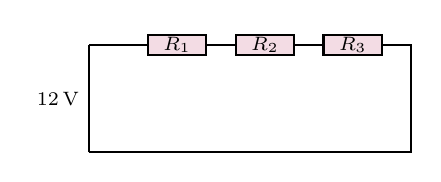
\begin{tikzpicture}[scale=0.62, every node/.style={font=\scriptsize}]
                \draw[thick] (0,0) -- (0,2.2);
                \draw[thick] (0,2.2) -- (1.2,2.2);
                \draw[thick,fill=cycfill] (1.2,2.0) rectangle (2.4,2.4);
                \node at (1.8,2.2) {$R_1$};
                \draw[thick] (2.4,2.2) -- (3.0,2.2);
                \draw[thick,fill=cycfill] (3.0,2.0) rectangle (4.2,2.4);
                \node at (3.6,2.2) {$R_2$};
                \draw[thick] (4.2,2.2) -- (4.8,2.2);
                \draw[thick,fill=cycfill] (4.8,2.0) rectangle (6.0,2.4);
                \node at (5.4,2.2) {$R_3$};
                \draw[thick] (6.0,2.2) -- (6.6,2.2) -- (6.6,0) -- (0,0);
                \node[left] at (0,1.1) {$12\,\mathrm{V}$};
            \end{tikzpicture}
            \end{center}
        \end{column}
    \end{columns}
\end{frame}

\begin{frame}{Putting It Together: Resistors in Parallel}
    \leavevmode
    \begin{columns}[t]
        \begin{column}{.5\textwidth}
            Components in \alert{parallel} are connected across the same
            two points, so each sees the \emph{same voltage}.
            \[
            \frac{1}{R_{\text{parallel}}} = \frac{1}{R_1} + \frac{1}{R_2} + \frac{1}{R_3}.
            \]
            \[
            I_k = \frac{V}{R_k}.
            \]
        \end{column}
        \begin{column}{.5\textwidth}
            \begin{center}
            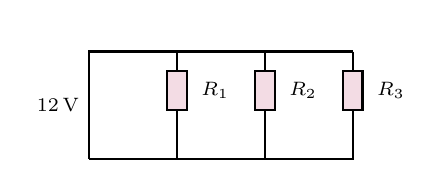
\begin{tikzpicture}[scale=0.62, every node/.style={font=\scriptsize}]
                \draw[thick] (0,0) -- (0,2.2) -- (1.8,2.2);
                \draw[thick,fill=cycfill] (1.6,1.0) rectangle (2.0,1.8);
                \node at (1.8,2.5) {};
                \node[right] at (2.1,1.4) {$R_1$};
                \draw[thick] (1.8,2.2) -- (1.8,1.8);
                \draw[thick] (1.8,1.0) -- (1.8,0);
                \draw[thick] (1.8,2.2) -- (3.6,2.2);
                \draw[thick,fill=cycfill] (3.4,1.0) rectangle (3.8,1.8);
                \node[right] at (3.9,1.4) {$R_2$};
                \draw[thick] (3.6,2.2) -- (3.6,1.8);
                \draw[thick] (3.6,1.0) -- (3.6,0);
                \draw[thick] (3.6,2.2) -- (5.4,2.2);
                \draw[thick,fill=cycfill] (5.2,1.0) rectangle (5.6,1.8);
                \node[right] at (5.7,1.4) {$R_3$};
                \draw[thick] (5.4,2.2) -- (5.4,1.8);
                \draw[thick] (5.4,1.0) -- (5.4,0) -- (0,0);
                \node[left] at (0,1.1) {$12\,\mathrm{V}$};
            \end{tikzpicture}
            \end{center}
        \end{column}
    \end{columns}
\end{frame}

\begin{frame}[fragile]{The Reason \texttt{input()} Belongs Here}
    \leavevmode
    Rather than typing component values into the program, we can ask for
    them with \texttt{input()}.

    \vspace{2mm}
    \begin{alertblock}{The essential point}
        \texttt{input()} \alert{always} returns a \textbf{string}, no
        matter what the user types.
    \end{alertblock}

\begin{lstlisting}
R = input("R1 (ohms): ")  # R is "100", not 100
R = R * 2                 # '100100' -- repetition, not math!

R = float(input("R1 (ohms): "))  # now R is 100.0
\end{lstlisting}

    \vspace{1mm}
    {\small Convert once, at the point of entry, and every later line can
    assume it has a number.}
\end{frame}

\begin{frame}[fragile]{Reading the Circuit Values}
    \leavevmode
\begin{lstlisting}
V  = float(input("Supply voltage V (volts): "))
R1 = float(input("R1 (ohms): "))
R2 = float(input("R2 (ohms): "))
R3 = float(input("R3 (ohms): "))

R_series = R1 + R2 + R3
I_series = V / R_series

R_parallel = 1 / (1/R1 + 1/R2 + 1/R3)
\end{lstlisting}

    \vspace{2mm}
    {\small Same three variables, two completely different formulas ---
    the data type conversion pattern is identical either way.}
\end{frame}

\begin{frame}[fragile]{Results: Series vs. Parallel}
    \leavevmode
    With $12\,\text{V}$, $R_1=100\,\Omega$, $R_2=220\,\Omega$,
    $R_3=330\,\Omega$:

    \begin{columns}[t]
        \begin{column}{.5\textwidth}
\begin{lstlisting}[style=skoutput]
--- Series ---
Total R:   650.0 ohms
Current:   18.462 mA
V(R1):     1.846 V
V(R2):     4.062 V
V(R3):     6.092 V
\end{lstlisting}
        \end{column}
        \begin{column}{.5\textwidth}
\begin{lstlisting}[style=skoutput]
--- Parallel ---
Total R:   56.90 ohms
Total I:   210.909 mA
I(R1):     120.000 mA
I(R2):     54.545 mA
I(R3):     36.364 mA
\end{lstlisting}
        \end{column}
    \end{columns}
\end{frame}

\begin{frame}{Check and Interpret}
    \leavevmode
    \begin{block}{Check: do the numbers add up?}
        \small
        \textbf{Series.} Voltage drops sum to the supply: $1.846 + 4.062
        + 6.092 = 12.000\,\text{V}$. \checkmark

        \vspace{1mm}
        \textbf{Parallel.} Branch currents sum to the total: $120.000 +
        54.545 + 36.364 = 210.909\,\text{mA}$. \checkmark
    \end{block}

    \vspace{3mm}
    \begin{alertblock}{Interpret: the surprising result}
        In series, total resistance ($650\,\Omega$) is \alert{larger}
        than any one resistor. In parallel, total resistance
        ($56.9\,\Omega$) is \alert{smaller} than the smallest resistor
        --- a useful sanity check for every parallel calculation.
    \end{alertblock}
\end{frame}

\begin{frame}[fragile]{When the User Types Something Unusable}
    \leavevmode
    \texttt{float()} raises an error if the text is not a number:

\begin{lstlisting}
V = float(input("Supply voltage V (volts): "))
# If the user types "12v" instead of "12":
# ValueError: could not convert string to float: '12v'
\end{lstlisting}

    \vspace{3mm}
    \begin{block}{This is the right behaviour}
        The program stops rather than continuing with a meaningless
        value. An unnoticed bad input is far worse than a halted
        program. Chapter 11 shows how to catch such errors and re-prompt
        instead of crashing.
    \end{block}
\end{frame}

%===============================================================================
\section{Editors and IDEs}
%===============================================================================

\begin{frame}{Code Editors vs. IDEs}
    \leavevmode
    Writing Python requires a text-editing tool. These fall into two
    categories:

    \vspace{3mm}
    \begin{columns}[t]
        \begin{column}{.5\textwidth}
            \begin{block}{Code editors}
                \small VS Code, Sublime Text, Vim, GNU Emacs, Atom,
                Notepad++.
            \end{block}
        \end{column}
        \begin{column}{.5\textwidth}
            \begin{block}{IDEs}
                \small PyCharm, \alert{Spyder}, Jupyter, IntelliJ IDEA.
            \end{block}
        \end{column}
    \end{columns}

    \vspace{3mm}
    \begin{alertblock}{What an IDE adds}
        It bundles essential tools --- editor, debugger, console,
        variable inspector --- into one interface, streamlining writing,
        testing, and debugging.
    \end{alertblock}
\end{frame}

\begin{frame}{Why Spyder for This Course}
    \leavevmode
    Spyder is particularly well suited to \alert{scientific and
    numerical} Python work:

    \vspace{2mm}
    \begin{itemize}
        \item Integrated scientific tools (NumPy, SciPy)
        \item A \alert{variable explorer} for easy data handling
        \item An IPython console for interactive coding
        \item Built-in plotting with Matplotlib
        \item Code completion, syntax highlighting, customizable layouts
    \end{itemize}
\end{frame}

\begin{frame}{The Three Panes of Spyder}
    \leavevmode
    \begin{columns}[t]
        \begin{column}{.33\textwidth}
            \begin{block}{Editor}
                \scriptsize Where you write and edit your Python scripts.
            \end{block}
        \end{column}
        \begin{column}{.33\textwidth}
            \begin{block}{Workspace}
                \scriptsize Variable Explorer --- an overview of
                variables and objects currently in memory.
            \end{block}
        \end{column}
        \begin{column}{.33\textwidth}
            \begin{block}{Console}
                \scriptsize Commands entered line by line, for testing
                snippets interactively.
            \end{block}
        \end{column}
    \end{columns}

    \vspace{4mm}
    {\small You can see your code, run it, and inspect the resulting
    values --- all at once.}
\end{frame}

\begin{frame}[fragile]{The \texttt{whos} Command}
    \leavevmode
    In Spyder's IPython Console, typing \texttt{whos} lists every
    current variable, with its type, size, and value:

\begin{lstlisting}
whos
\end{lstlisting}

    \vspace{3mm}
    \begin{block}{Why this matters}
        It is the fastest way to check \alert{what Python actually
        thinks} a variable's type and value are --- especially useful
        when a calculation gives an unexpected result.
    \end{block}
\end{frame}

%===============================================================================
\section{Summary}
%===============================================================================

\begin{frame}{What You Should Take Away}
    \leavevmode
    \small
    \begin{itemize}
        \item A language has \textbf{syntax} (grammar), \textbf{variables}
              (nouns), and \textbf{operations} (verbs).
        \item Python uses \textbf{dynamic typing} --- it infers a
              variable's type at runtime from the assigned value.
        \item Five \textbf{scalar} types: \texttt{int}, \texttt{float},
              \texttt{str}, \texttt{bool}, \texttt{None}.
        \item Convert explicitly with \texttt{int()}, \texttt{float()},
              \texttt{str()}, \texttt{bool()} --- except \texttt{None},
              which can only be assigned directly.
    \end{itemize}
\end{frame}

\begin{frame}{What You Should Take Away (continued)}
    \leavevmode
    \small
    \begin{itemize}
        \item Translating formulas needs care: write \texttt{*}
              explicitly, use \texttt{**} for powers (never
              \texttt{\^{}}), parenthesize every implied grouping, and
              convert degrees to radians before calling \texttt{math}'s
              trig functions.
        \item \texttt{input()} \alert{always} returns a string --- wrap
              it in \texttt{float()} or \texttt{int()} before using it
              in arithmetic.
        \item Series resistors add; parallel resistors' reciprocals add,
              giving a total \emph{smaller} than the smallest resistor.
        \item An \textbf{IDE} like Spyder combines an editor, console,
              and variable explorer in one place.
    \end{itemize}
\end{frame}

\begin{frame}{Where This Is Going}
    \leavevmode
    \small
    This chapter built the foundation: variables, scalar types,
    conversion, and the editor you will work in.

    \vspace{3mm}
    \begin{itemize}
        \item Chapter 3 builds on these basic types: complex numbers,
              strings, and Python's collection types, together with the
              engineering units a measured value carries.
        \item Every later program is still just variables and
              operations --- now with richer types to work with.
    \end{itemize}

    \vspace{4mm}
    \begin{center}
        \large\color{primary}\textbf{Next: Numbers, Variables and Units}
    \end{center}
\end{frame}

\end{document}
